\documentclass{ctexart}
\usepackage[a4paper, margin=1.5cm]{geometry}
\linespread{1.5}
\usepackage{amsmath, amssymb}
\usepackage{graphicx}
\usepackage{booktabs}
\usepackage{caption}
\usepackage{float}
\DeclareMathOperator*{\argmin}{argmin}
\title{论文标题}
\date{}
\author{马文杰\and 李传浩\and 张可欣}
\begin{document}
\maketitle
\begin{abstract}
本文针对\textbf{<题目主题>}问题展开研究。首先对附件数据进行预处理与统计分析，提出了\ldots\ 模型。

针对问题一，本文\ldots（简述方法），得到\ldots（简述关键结果）。

针对问题二，本文\ldots（简述方法），得到\ldots（简述关键结果）。

针对问题三，本文\ldots（简述方法），得到\ldots（简述关键结果）。

针对问题四，本文\ldots（简述方法），得到\ldots（简述关键结果）。

综上所述，本文所建立的模型\ldots（总结模型适用性与优点）。

\vspace{0.3em}
\noindent\textbf{关键词：}关键字1；关键字2；关键字3；关键字4
\end{abstract}
\section{问题重述}
\section{问题分析}
\section{提出假设}
\section{问题一：算力需求分析与短期预测}
\subsection{图形处理器需求统计分析}
对工作负载轨迹中的 50000 个人工智能任务，按区域与任务类型统计其图形处理器需求分布，结果如表~\ref{tab:gpu_type}、表~\ref{tab:gpu_region} 所示。

\begin{table}[H]
	\centering
	\caption{不同任务类型的 GPU 需求统计}
	\label{tab:gpu_type}
	\begin{tabular}{lcccc}
		\toprule
		任务类型 & 任务数 & 需求量均值 & 最大值 & GPU-小时总量 \\
		\midrule
		实时推理任务 & 16724 & 4.0 & 7 & 228150 \\
		批量推理任务 & 16717 & 13.5 & 23 & 769098 \\
		人工智能训练任务 & 16559 & 71.3 & 127 & 4023539 \\
		\bottomrule
	\end{tabular}
\end{table}

三类任务的需求特征分层明显：实时推理任务单任务图形处理器需求量小、数量多、时延敏感；人工智能训练任务单任务需求量最大，是算力消耗的主体，其图形处理器-小时总量约占全部任务的 80\%；批量推理任务介于两者之间。

\begin{table}[H]
	\centering
	\caption{不同区域的 GPU 需求统计}
	\label{tab:gpu_region}
	\begin{tabular}{lcccc}
		\toprule
		区域 & 任务数 & 需求量均值 & GPU-小时总量 \\
		\midrule
		区域A & 10062 & 13.1 & 448452 \\
		区域B & 9200 & 13.8 & 430758 \\
		区域C & 7559 & 14.6 & 374934 \\
		区域D & 9560 & 47.6 & 1548858 \\
		区域E & 6912 & 46.9 & 1087748 \\
		区域F & 6707 & 48.5 & 1130035 \\
		\bottomrule
	\end{tabular}
\end{table}

分区域看，东部高负荷区域 A、B、C 以实时推理与批量推理任务为主，任务数量大但单任务需求小，需求量均值约 13–15；西部区域 D、E、F 承接大量人工智能训练任务，单任务需求大，需求量均值约 47–49，其中区域 D 的图形处理器-小时总量最大（约 155 万）。上述特征表明：训练任务是跨区域调度与新能源协同的主要调节对象，东部存在较大的可迁移算力空间，与后文基础调度及碳感知调度的分析结果一致。分区域、分任务类型的图形处理器需求分布如图 1 所示。

\subsection{算力需求短期预测模型}

赛题要求利用历史到达数据构建短期预测模型，为第 2376–2399 小时的调度提供前瞻性的图形处理器需求输入。小时级图形处理器需求序列具有较强的波动性，传统时间序列模型（如 ETS、ARIMA）对该类序列的预测精度有限。\textbf{文献研究表明，变分模态分解（VMD）等自适应信号分解方法可将原始序列拆分为若干相对平稳的模态分量，对各分量分别建模预测、最后叠加得到整体预测，从而降低序列复杂度、提升预测精度（张行等，2026；胡宏等，2026）。}受此思路启发，本文在 R 环境下以自适应集合经验模态分解（CEEMDAN）实现信号分解。

\textbf{自适应集合经验模态分解（CEEMDAN）模型}

CEEMDAN 在经验模态分解（EMD）的基础上，通过向残差信号逐次叠加自适应高斯白噪声并进行集合平均以抑制模态混叠，将原始图形处理器需求序列 $x(t)$ 分解为 $K$ 个模态分量 $\mathrm{IMF}_k(t)$ 与残差项 $r(t)$：
\begin{equation}
	x(t)=\sum_{k=1}^{K}\mathrm{IMF}_k(t)+r(t)
\end{equation}

与变分模态分解（VMD）等同属自适应信号分解方法，CEEMDAN 无需预设中心频率，依靠迭代筛分自适应确定各模态分量，更适用于近似平稳且无明显周期结构的波动序列。将所得分量按频率特征划分为低频趋势分量、中频波动分量与高频随机分量，分别采用适用的模型预测后叠加重构：

\begin{equation}
    \hat x(t+h)=\sum_{k\in\mathcal{L}}\widehat{\mathrm{IMF}}_k(t+h)+\sum_{k\in\mathcal{M}}\widehat{\mathrm{IMF}}_k(t+h)+\sum_{k\in\mathcal{H}}\widehat{\mathrm{IMF}}_k(t+h)
\end{equation}
其中 $\mathcal{L}$、$\mathcal{M}$、$\mathcal{H}$ 分别为低频、中频、高频分量下标集合。

为量化预测精度，本文采用均方根误差（RMSE）、平均绝对误差（MAE）与平均绝对百分比误差（MAPE）三项指标，其定义为：
\begin{align}
\mathrm{RMSE}&=\sqrt{\frac{1}{N}\sum_{t=1}^{N}\big(y_t-\hat y_t\big)^2},\\
\mathrm{MAE}&=\frac{1}{N}\sum_{t=1}^{N}\big|y_t-\hat y_t\big|,\\
\mathrm{MAPE}&=\frac{1}{N}\sum_{t=1}^{N}\frac{\big|y_t-\hat y_t\big|}{y_t}\times 100\%
\end{align}
其中 $y_t$ 为第 $t$ 小时图形处理器需求实际值，$\hat y_t$ 为模型预测值，$N=24$ 为预测步数。以第 0--2375 小时逐时图形处理器总需求为训练数据，向前预测第 2376--2399 小时共 24 步，与测试集实际值比较，结果如表~\ref{tab:model_cmp} 所示。

\subsection{组合预测与最终模型选择}
% 此处写 ETS、ARIMA 及组合预测的实验对比。新建对比表时请用 \label{tab:model_cmp}，以匹配上文表~\ref{tab:model_cmp} 的引用……

\subsection{基础算力调度模型}
以最小化任务总开工延迟与迁移惩罚之和为目标，建立混合整数规划模型，目标函数与约束如下：
\begin{equation}
	\argmin_{s_{i},y_{i,r}}\ \sum_{i\in\mathcal{I}}\big(s_i-a_i\big)+\theta\sum_{i\in\mathcal{I}}\sum_{r\in\mathcal{R}\setminus\{o_i\}}y_{i,r}
\end{equation}
% 此处补充约束条件（容量、时延、完成时限）与求解结果……

\begin{figure}[H]
	\centering
	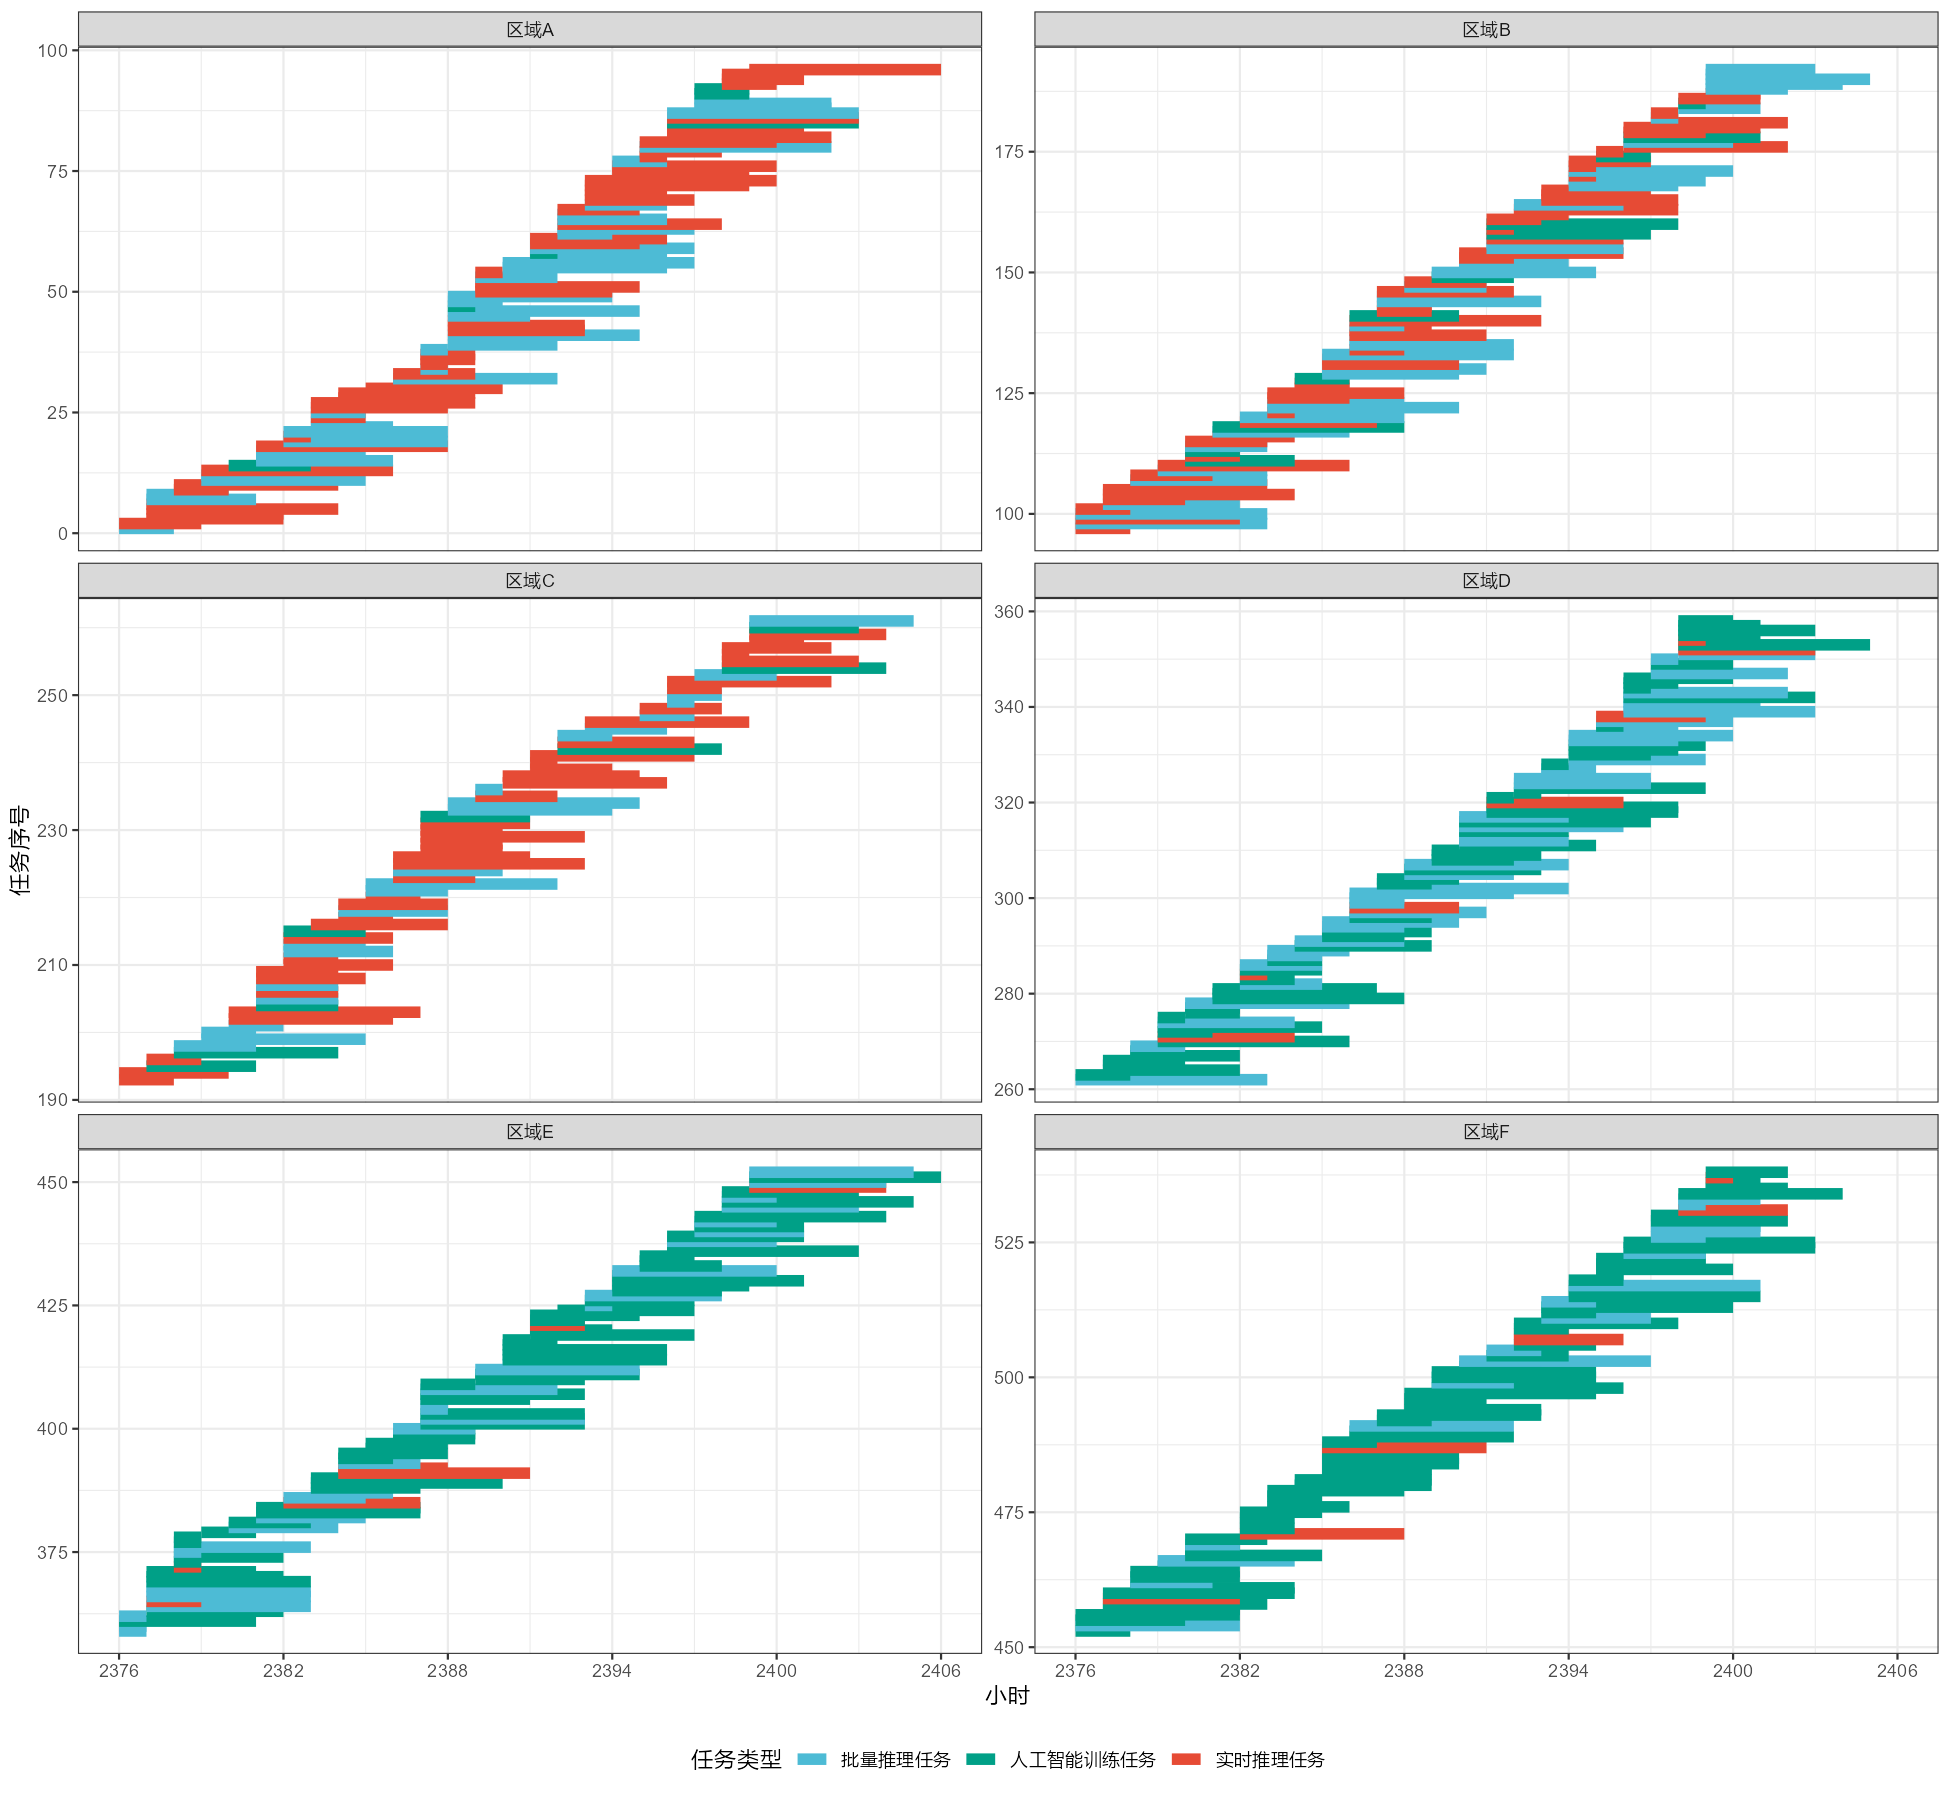
\includegraphics[width=0.9\textwidth]{../解答/1-第一题/甘特图_基础调度.png}
	\caption{第 2376--2406 小时基础调度甘特图}
	\label{fig:gantt}
\end{figure}

\begin{figure}[H]
	\centering
	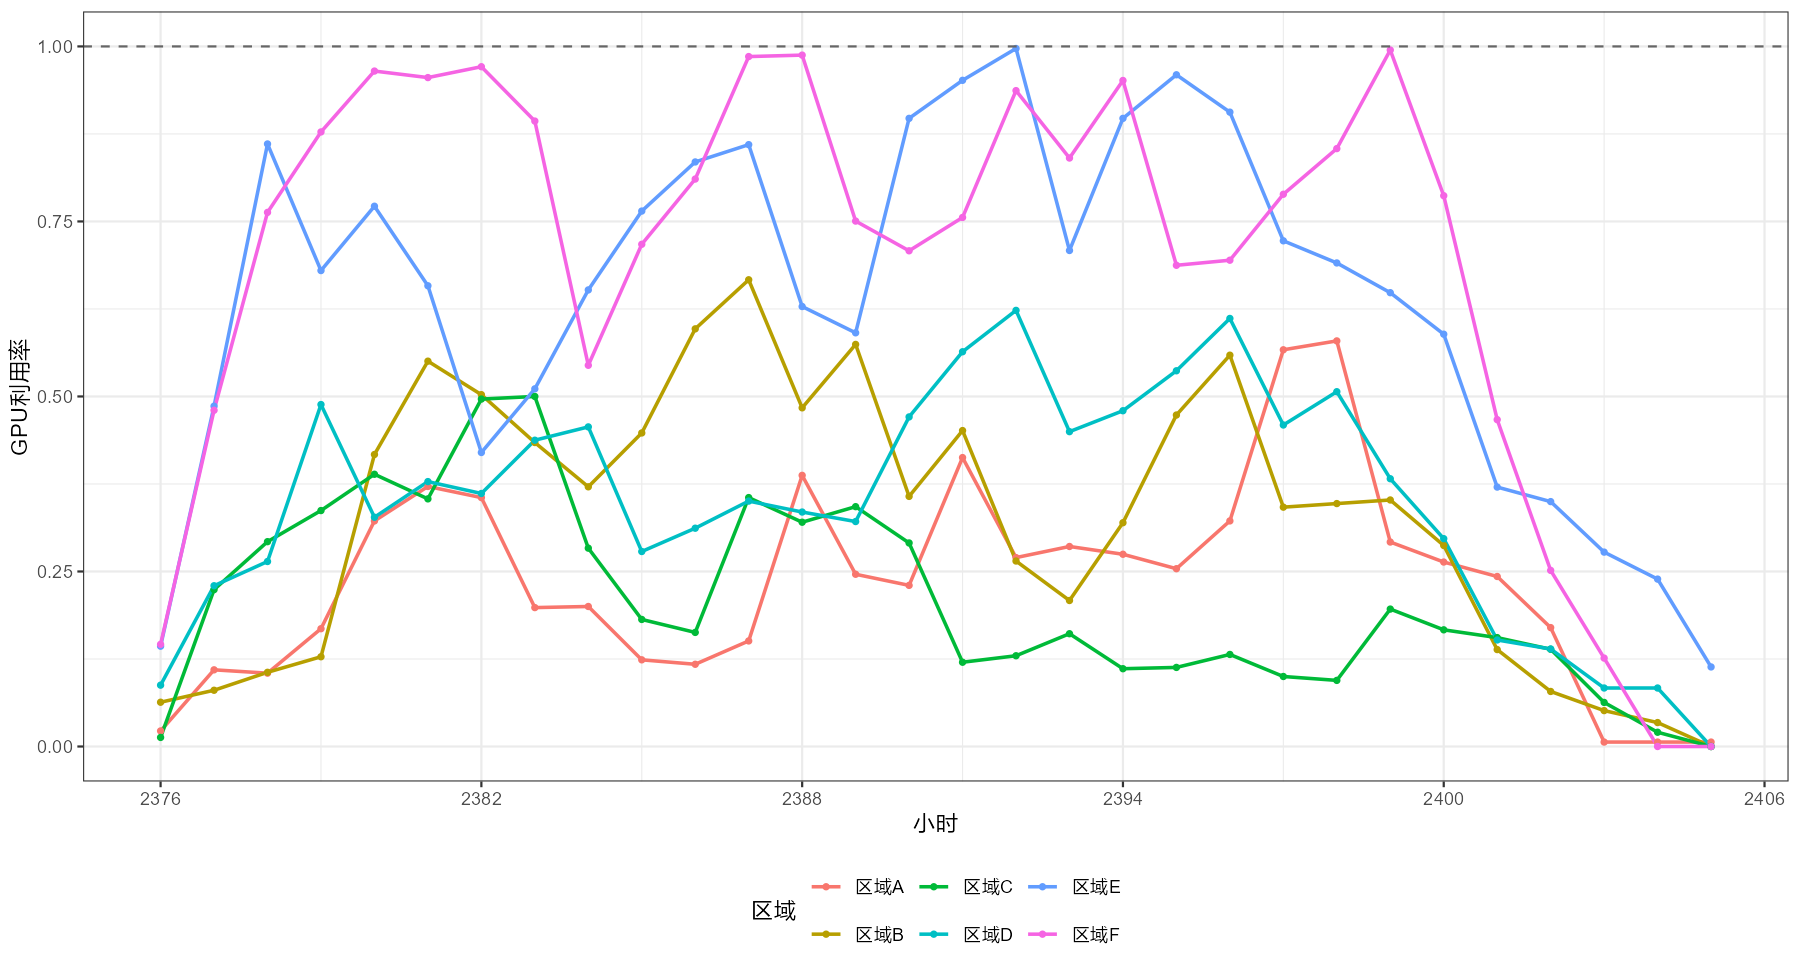
\includegraphics[width=0.9\textwidth]{../解答/1-第一题/GPU利用率_区域.png}
	\caption{六区域逐时 GPU 利用率}
	\label{fig:gpu_util}
\end{figure}

% \section{问题2模型}   % 待写问题二时取消注释
%\section{问题3模型}
%\section{问题4模型}
%\section{误差}
%\section{优缺点}
\end{document}